\documentclass[11pt,compress,t,notes=noshow]{beamer}\usepackage[]{graphicx}\usepackage[]{color}

\makeatletter
\def\maxwidth{ %
  \ifdim\Gin@nat@width>\linewidth
    \linewidth
  \else
    \Gin@nat@width
  \fi
}
\makeatother

\definecolor{fgcolor}{rgb}{0.345, 0.345, 0.345}
\newcommand{\hlnum}[1]{\textcolor[rgb]{0.686,0.059,0.569}{#1}}%
\newcommand{\hlstr}[1]{\textcolor[rgb]{0.192,0.494,0.8}{#1}}%
\newcommand{\hlcom}[1]{\textcolor[rgb]{0.678,0.584,0.686}{\textit{#1}}}%
\newcommand{\hlopt}[1]{\textcolor[rgb]{0,0,0}{#1}}%
\newcommand{\hlstd}[1]{\textcolor[rgb]{0.345,0.345,0.345}{#1}}%
\newcommand{\hlkwa}[1]{\textcolor[rgb]{0.161,0.373,0.58}{\textbf{#1}}}%
\newcommand{\hlkwb}[1]{\textcolor[rgb]{0.69,0.353,0.396}{#1}}%
\newcommand{\hlkwc}[1]{\textcolor[rgb]{0.333,0.667,0.333}{#1}}%
\newcommand{\hlkwd}[1]{\textcolor[rgb]{0.737,0.353,0.396}{\textbf{#1}}}%
\let\hlipl\hlkwb

\usepackage{framed}
\makeatletter
\newenvironment{kframe}{%
 \def\at@end@of@kframe{}%
 \ifinner\ifhmode%
  \def\at@end@of@kframe{\end{minipage}}%
  \begin{minipage}{\columnwidth}%
 \fi\fi%
 \def\FrameCommand##1{\hskip\@totalleftmargin \hskip-\fboxsep
 \colorbox{shadecolor}{##1}\hskip-\fboxsep
     \hskip-\linewidth \hskip-\@totalleftmargin \hskip\columnwidth}%
 \MakeFramed {\advance\hsize-\width
   \@totalleftmargin\z@ \linewidth\hsize
   \@setminipage}}%
 {\par\unskip\endMakeFramed%
 \at@end@of@kframe}
\makeatother

\definecolor{shadecolor}{rgb}{.97, .97, .97}
\definecolor{messagecolor}{rgb}{0, 0, 0}
\definecolor{warningcolor}{rgb}{1, 0, 1}
\definecolor{errorcolor}{rgb}{1, 0, 0}
\definecolor{code}{rgb}{0.97, 0.96, 1.0}
\newenvironment{knitrout}{}{} % an empty environment to be redefined in TeX

\usepackage{alltt}
\usepackage[utf8]{inputenc}
\usepackage[ngerman]{babel}
\usepackage{dsfont}
\usepackage{verbatim}
\usepackage{amsmath}
\usepackage{amsfonts}
\usepackage{mathtools}
\usepackage{csquotes}
\usepackage{cmbright}
\usepackage{multirow}
\usepackage{longtable}
\usepackage{enumerate}
\usepackage[absolute,overlay]{textpos}
\usepackage{psfrag}
\usepackage{algorithm}
\usepackage{algpseudocode}
\usepackage{eqnarray}
\usepackage{bytefield}
\usepackage{animate}
\usepackage{tikz}
\usetikzlibrary{shapes,matrix,positioning,chains,arrows,shadows,decorations.pathmorphing,fit,backgrounds}
\usepackage{adjustbox}
\usepackage{colortbl}
\usepackage{tabularx} % for tables (incl. \hline)
\usepackage{arydshln} % Load after array, longtable, colortab and/or colortbl , otherwise problems with \hline in tabular env
\usepackage{etex} %increase registers for \dimenS to more than 256, otherwise we get "No room for a new \dimen"
\usepackage{graphicx}
\usepackage{booktabs} %used in epr lectures
\usepackage{bm} % bold greek letters
\usepackage{hyperref} % url citing
\usepackage{blkarray} % block arrays
\usepackage{listings} % block of code
\usepackage{xcolor} %colored math symbols
\usepackage{pgffor}
\usepackage{verbatimbox}
\usepackage{xcolor}

%some colors
\definecolor{checkgreen}{HTML}{18A126}
\definecolor{errorred}{HTML}{FF0000}
\definecolor{blockbg}{HTML}{F7F7F7}
\definecolor{gray}{HTML}{A0A0A0}

% basic latex stuff
\newcommand{\col}{\par\colorbox{code}{\parbox{\textwidth}{\theverbbox}}\par}
\newcommand{\eg}{e.\,g.\xspace} %for example
\newcommand{\ie}{i.\,e.\xspace} %that is to say...
\newcommand{\pkg}[1]{{\fontseries{b}\selectfont #1}} %fontstyle for R packages
\newcommand{\lz}{\vspace{0.5cm}} %vertical space
\newcommand{\oneliner}[1] % Oneliner for important statements
{\begin{block}{}\begin{center}\begin{Large}#1\end{Large}\end{center}\end{block}}
\def\SpAr{\quad \Rightarrow \quad}

%new environments
\newenvironment{vbframe}  %frame with breaks and verbatim
{
 \begin{frame}[containsverbatim,allowframebreaks]
}
{
\end{frame}
}

\newenvironment{vframe}  %frame with verbatim without breaks (to avoid numbering one slided frames)
{
 \begin{frame}[containsverbatim]
}
{
\end{frame}
}

\newenvironment{blocki}[1]   % itemize block
{
 \begin{block}{#1}\begin{itemize}
}
{
\end{itemize}\end{block}
}

\newenvironment{fragileframe}[2]{  %fragile frame with framebreaks
\begin{frame}[allowframebreaks, fragile, environment = fragileframe]
\frametitle{#1}
#2}
{\end{frame}}

\newcommand{\myframe}[2]{  %short for frame with framebreaks
\begin{frame}[allowframebreaks]
\frametitle{#1}
#2
\end{frame}}

\usepackage{../../style/lmu-lecture}

\let\code=\texttt
\let\proglang=\textsf

\setkeys{Gin}{width=0.9\textwidth}

\usepackage{tikz}
\usetikzlibrary{shapes,arrows,snakes, calc}

% Define block styles
\tikzstyle{decision} = [diamond, draw, text width=6em, text badly centered, node distance=4cm, inner sep=0pt]
\tikzstyle{decision2} = [diamond, draw, fill=customgreen!35, text width=6em, text badly centered, node distance=4cm, inner sep=0pt]

\tikzstyle{block} = [rectangle, draw, text width=14em, text centered, rounded corners, node distance=3cm, minimum height=4em]
\tikzstyle{line} = [draw, -latex']
\tikzstyle{cloud} = [draw, ellipse, node distance=3cm, minimum height=2em]

\title{Introduction to Deep Learning}
\author{Bernd Bischl}
\institute{Department of Statistics -- LMU Munich}
\date{WS 2021/2022}

\setbeamertemplate{frametitle}{\expandafter\uppercase\expandafter\insertframetitle}

\IfFileExists{upquote.sty}{\usepackage{upquote}}{}
\input{../../latex-math/basic-math}
\input{../../latex-math/basic-ml}
\input{../../latex-math/ml-nn}

\newcommand{\titlefigure}{plots/xcorrel_animations/conv_xcorrel.png}
%modify picture
\newcommand{\learninggoals}{
  \item Convolution vs. Cross-Correlation
}

\title{Deep Learning}
\date{}



\begin{document}

\lecturechapter{Convolutions - Mathematical Perspective}
\lecture{I2DL}
%%%%%%%%%%%%%%%%%%%%%%%%%%%%%%%%%%%%%%%%%%%%%%%%%%%%%%%%%%%%%%%%%%

%%%%%%%%%%%%%%%%%%%%%%%%%%%%%%%%%%%%%%%%%%%%%%%%%%%%%%%%%%%%%%%%%%
\begin{vbframe}{Convolutions : A Deeper Look}
    \begin{itemize}
        \item CNNs borrow their name from a mathematical operation termed \textbf{convolution} that originates in Signal Processing.
        \item Basic understanding of this concept and related operations improves the understanding of the CNN functionality.
        \item Still, there are successful practitioners that never heard of these concepts.
        \item The following should provide exactly this fundamental understanding of convolutions.
    \end{itemize}
\framebreak
    \begin{itemize}
        \item Definition: \\
            \begin{equation*}
                \begin{split}
                    h(i) &= (f \ast g)(i) = \int f(x)g(i-x)dx \\
                    \text{where } f(x)&: \text{input function} \\
                    \text{and } g(x)&: \text{weighting function, kernel} \\
                    \text{and } h(i)&: \text{output function, feature map elements}
          %          \text{for } f, g &\in \mathcal{R}^{d} \mapsto h \in \mathcal{R}^{d}
                \end{split}
            \end{equation*}
        \item Intuition 1: weighted smoothing of $f(x)$ with weighting function $g(x)$. 
        \item Intuition 2: filter function $g(x)$ filters features $h(i)$ from input signal $f(x)$.
    \end{itemize}
\end{vbframe}    

%%%%%%%%%%%%%%%%%%%%%%%%%%%%%%%%%%%%%%%%%%%%%%%%%%%%%%%%%%%%%%%%%%
%%%%%%%%%%%%%%%%%%%%%%%%%%%%%%%%%%%%%%%%%%%%%%%%%%%%%%%%%%%%%%%%%%
\begin{vbframe}{1D Convolution Animation}
    \begin{figure}
    \centering
    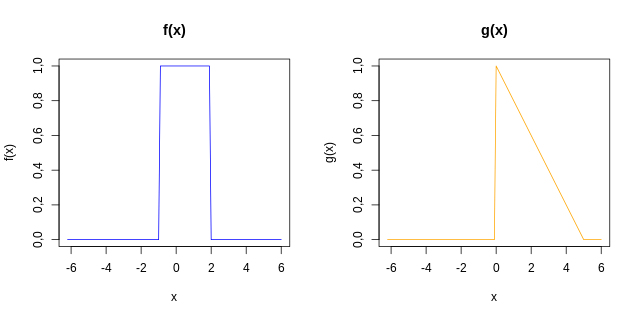
\includegraphics[width=10cm]{plots/conv_animations/conv_static.png}
    \end{figure}
    \begin{equation*}
        f(x)=
        \begin{cases}
            1, & \text{if } x\in [-1, 2]\\
            0, & \text{otherwise}
        \end{cases}
        \qquad
        g(x)=
        \begin{cases}
            1 - 0.2*|x|, & \text{if } x > 0\\
            0, & \text{otherwise}
        \end{cases}
    \end{equation*}
\end{vbframe}

\begin{vbframe}{1D Convolution Animation}
    \begin{figure}
    \centering
    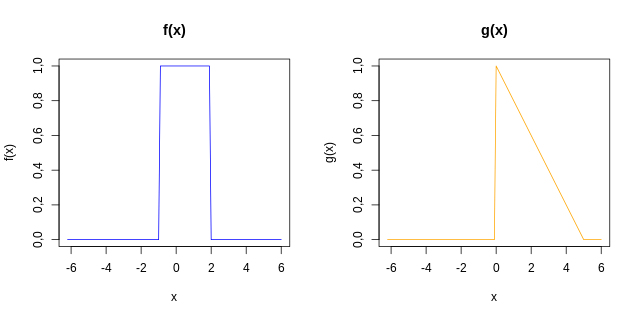
\includegraphics[width=10cm]{plots/conv_animations/conv_static.png}
    \end{figure}
    Kernel is flipped due to the negative iterator in $$h(i) = \int_{x = -\infty}^{\infty} f(x)g(i-x)$$
\end{vbframe}

 \frame{
 \frametitle{1D Convolution Animation}
     \center
         \only<1>{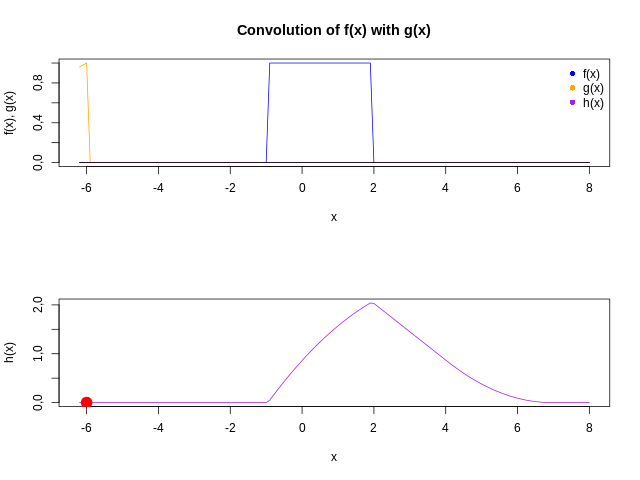
\includegraphics[width=11cm]{plots/conv_animations/conv_anim_1.png}}%
         \only<2>{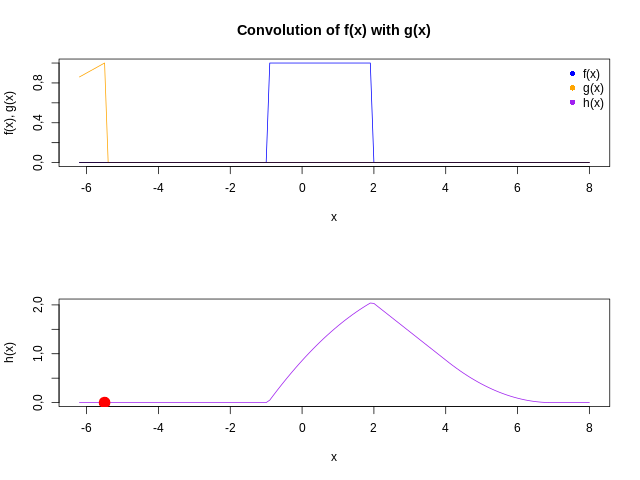
\includegraphics[width=11cm]{plots/conv_animations/conv_anim_2.png}}%
         \only<3>{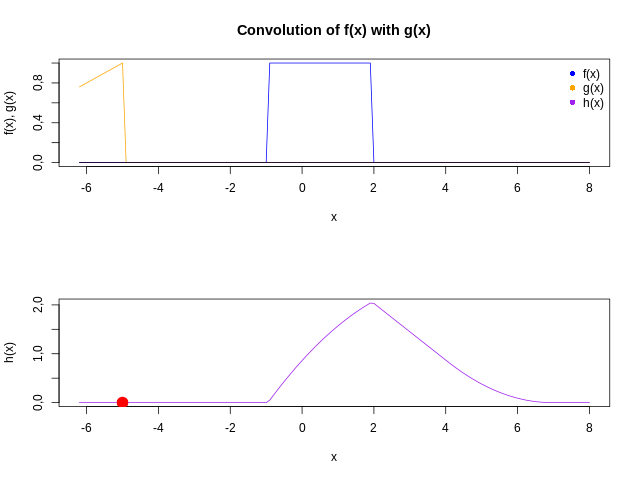
\includegraphics[width=11cm]{plots/conv_animations/conv_anim_3.png}}%
         \only<4>{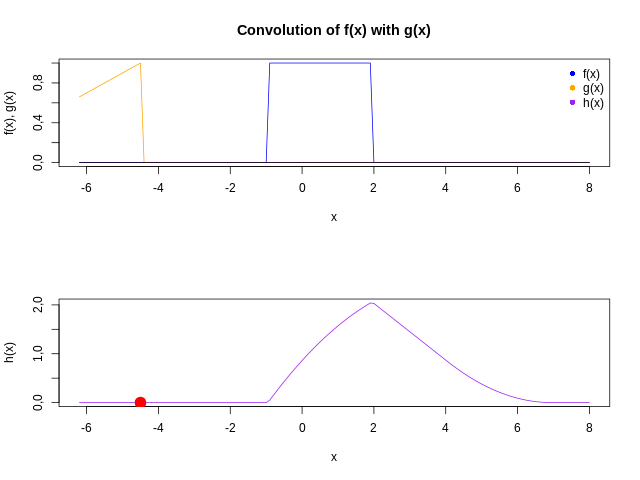
\includegraphics[width=11cm]{plots/conv_animations/conv_anim_4.png}}%
         \only<5>{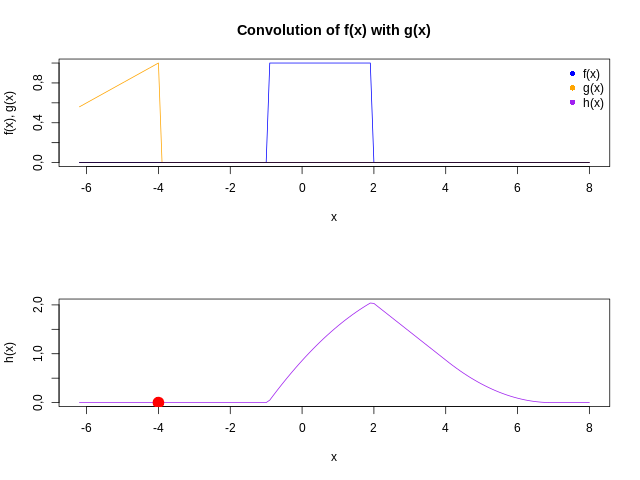
\includegraphics[width=11cm]{plots/conv_animations/conv_anim_5.png}}%
         \only<6>{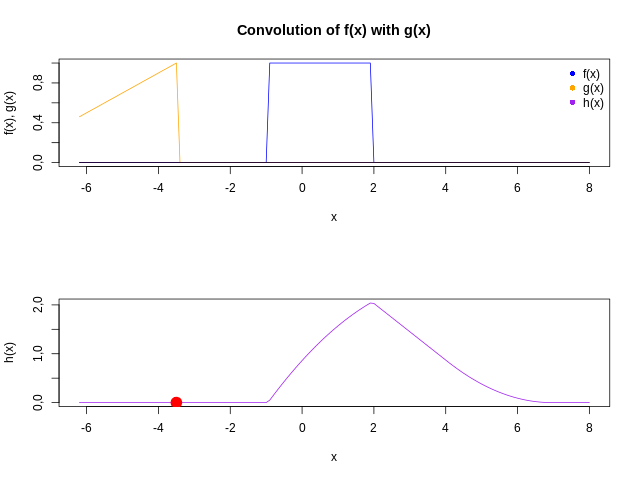
\includegraphics[width=11cm]{plots/conv_animations/conv_anim_6.png}}%
         \only<7>{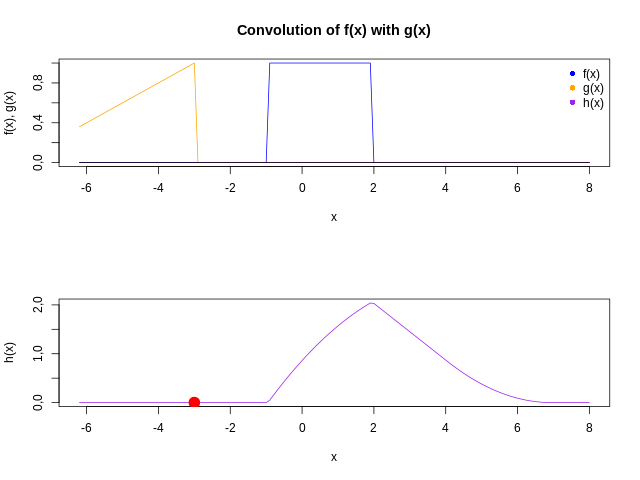
\includegraphics[width=11cm]{plots/conv_animations/conv_anim_7.png}}%
         \only<8>{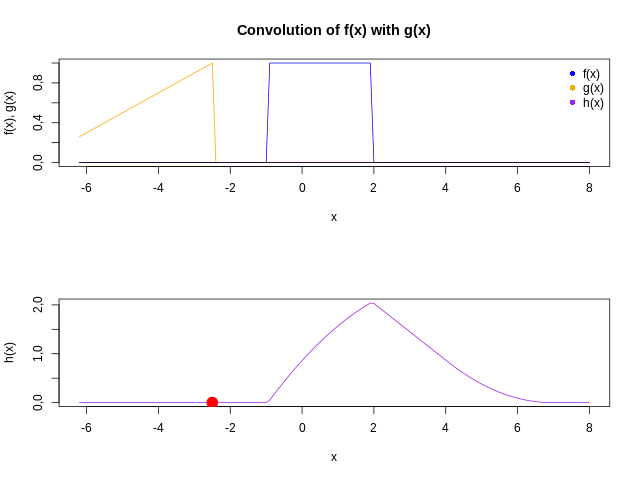
\includegraphics[width=11cm]{plots/conv_animations/conv_anim_8.png}}%
         \only<9>{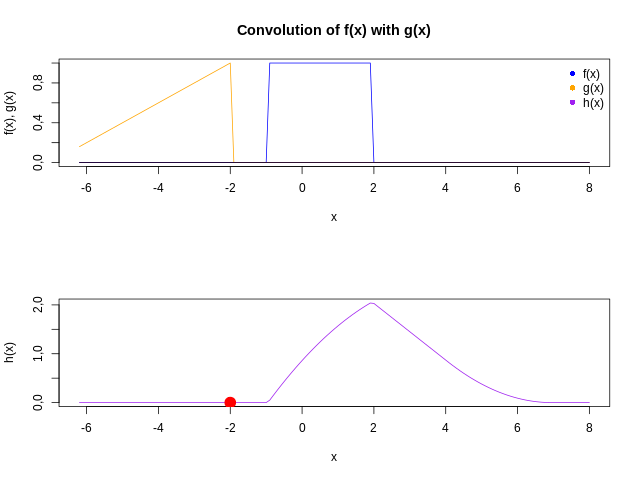
\includegraphics[width=11cm]{plots/conv_animations/conv_anim_9.png}}%
         \only<10>{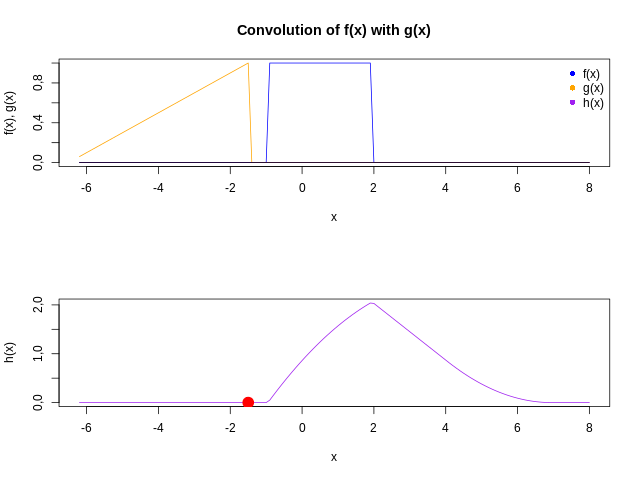
\includegraphics[width=11cm]{plots/conv_animations/conv_anim_10.png}}%
         \only<11>{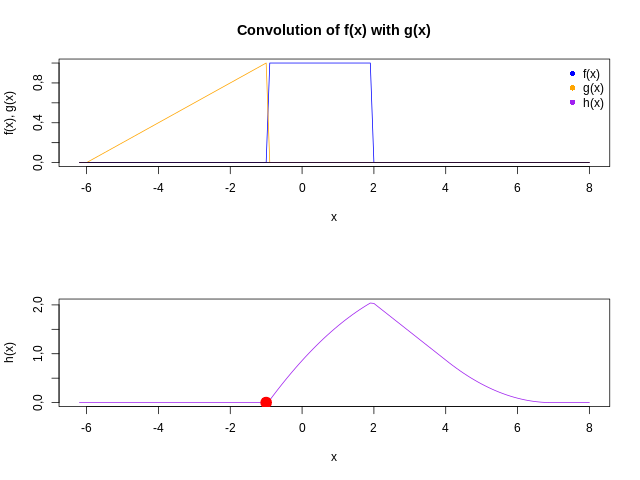
\includegraphics[width=11cm]{plots/conv_animations/conv_anim_11.png}}%
         \only<12>{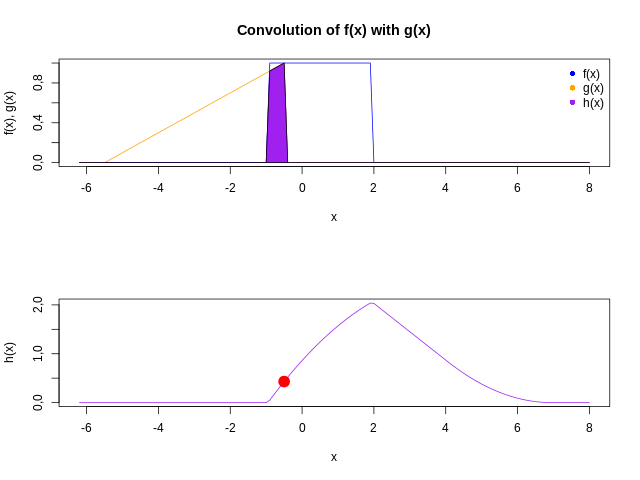
\includegraphics[width=11cm]{plots/conv_animations/conv_anim_12.png}}%
         \only<13>{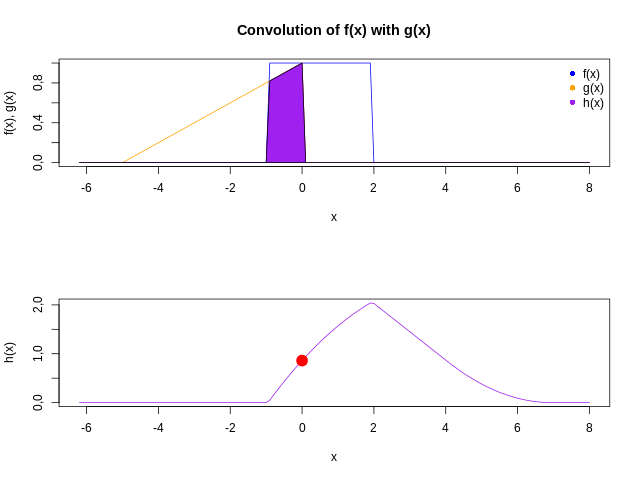
\includegraphics[width=11cm]{plots/conv_animations/conv_anim_13.png}}%
         \only<14>{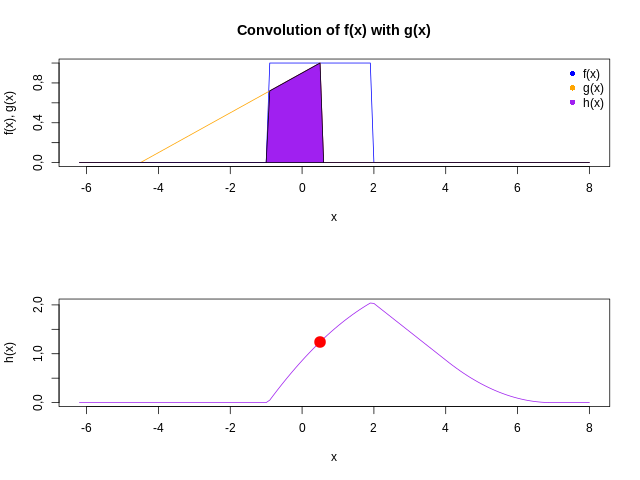
\includegraphics[width=11cm]{plots/conv_animations/conv_anim_14.png}}%
         \only<15>{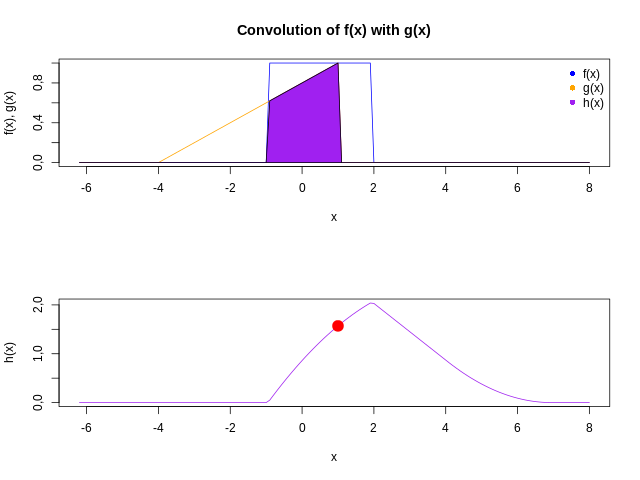
\includegraphics[width=11cm]{plots/conv_animations/conv_anim_15.png}}%
         \only<16>{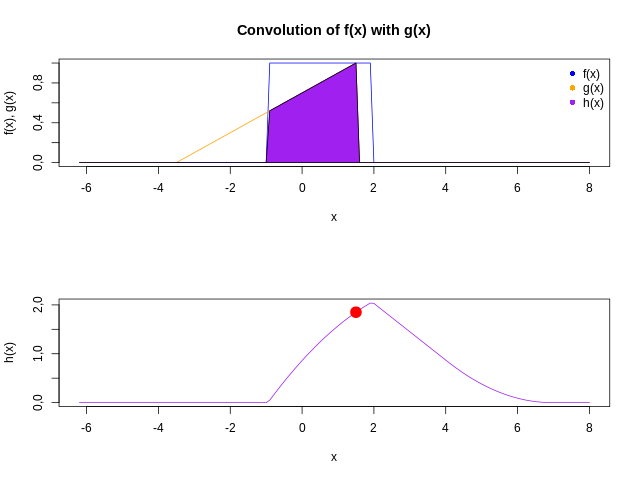
\includegraphics[width=11cm]{plots/conv_animations/conv_anim_16.png}}%
         \only<17>{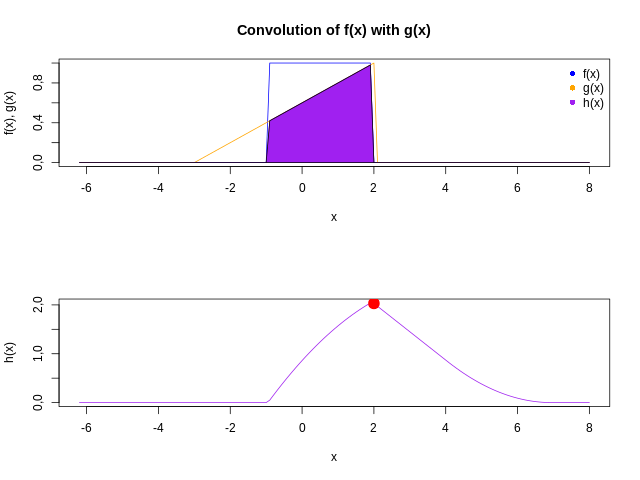
\includegraphics[width=11cm]{plots/conv_animations/conv_anim_17.png}}%
         \only<18>{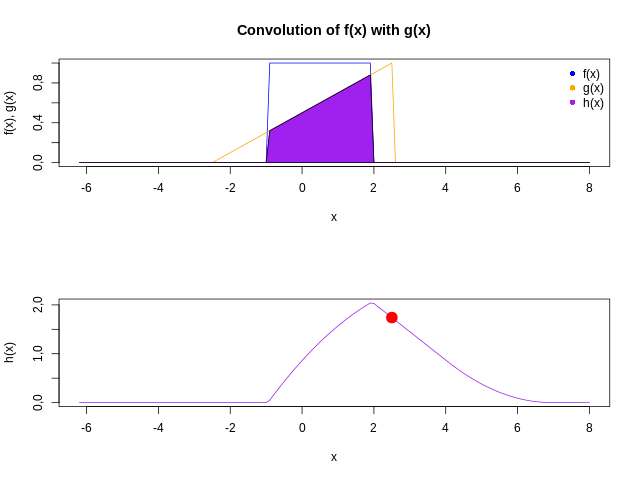
\includegraphics[width=11cm]{plots/conv_animations/conv_anim_18.png}}%
         \only<19>{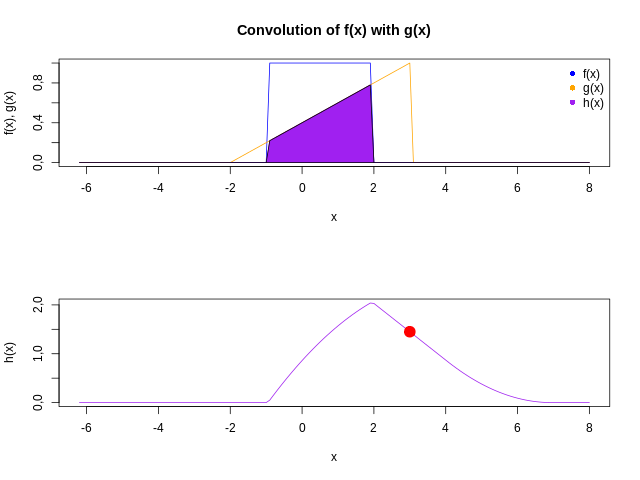
\includegraphics[width=11cm]{plots/conv_animations/conv_anim_19.png}}%
         \only<20>{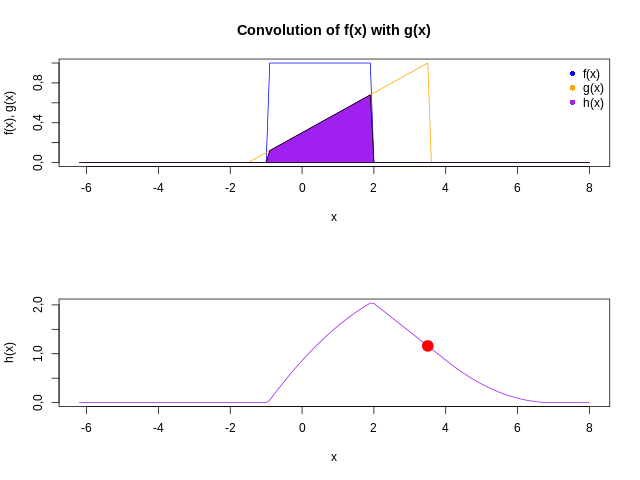
\includegraphics[width=11cm]{plots/conv_animations/conv_anim_20.png}}%
         \only<21>{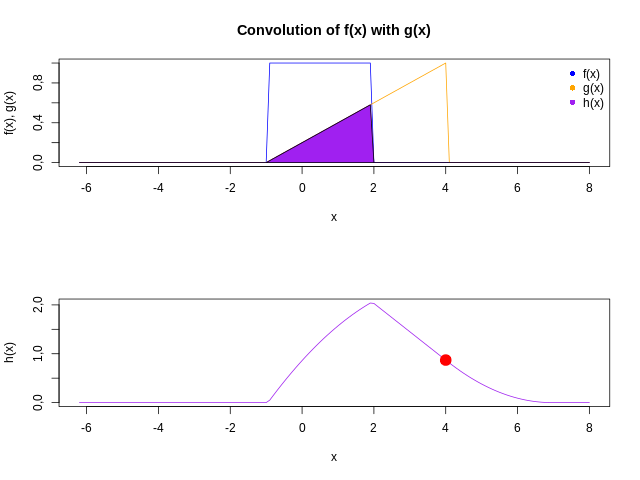
\includegraphics[width=11cm]{plots/conv_animations/conv_anim_21.png}}%
         \only<22>{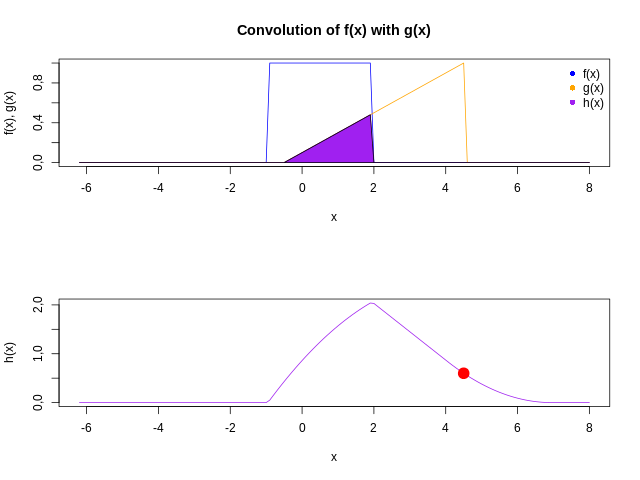
\includegraphics[width=11cm]{plots/conv_animations/conv_anim_22.png}}%
         \only<23>{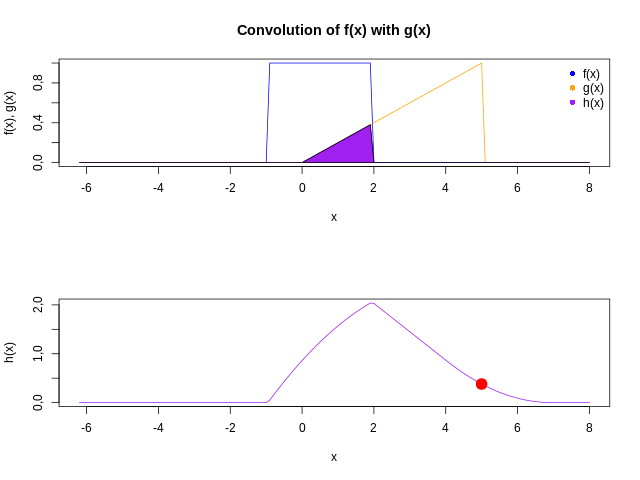
\includegraphics[width=11cm]{plots/conv_animations/conv_anim_23.png}}%
         \only<24>{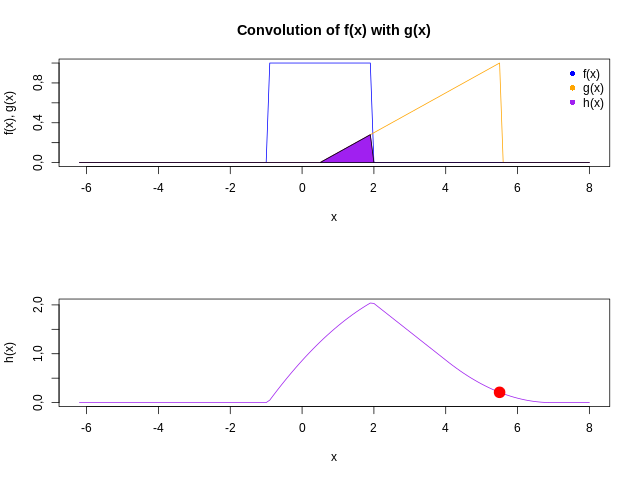
\includegraphics[width=11cm]{plots/conv_animations/conv_anim_24.png}}%
         \only<25>{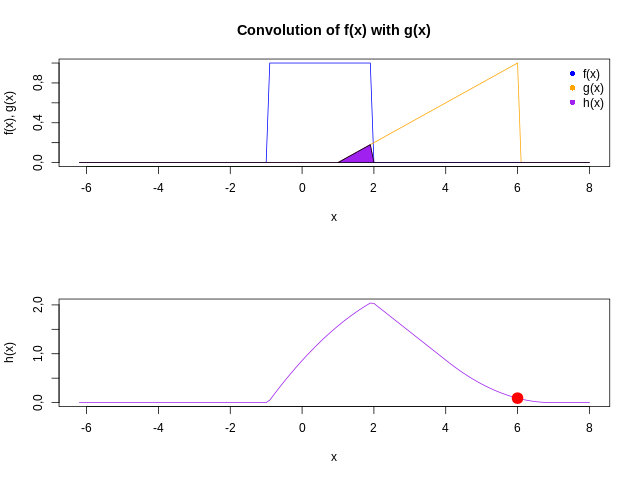
\includegraphics[width=11cm]{plots/conv_animations/conv_anim_25.png}}%
         \only<26>{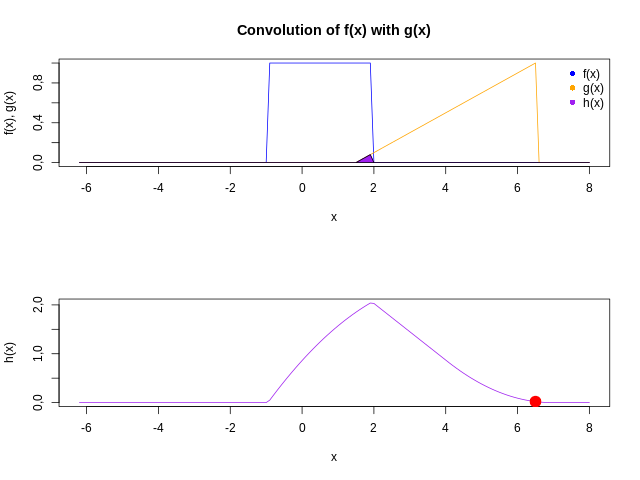
\includegraphics[width=11cm]{plots/conv_animations/conv_anim_26.png}}%
         \only<27>{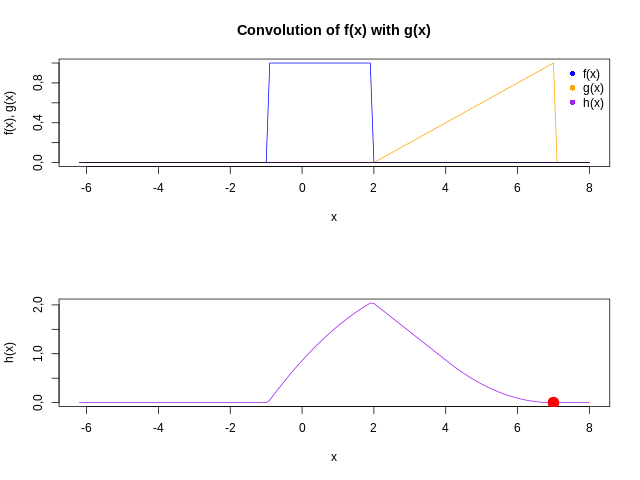
\includegraphics[width=11cm]{plots/conv_animations/conv_anim_27.png}}%
         \only<28>{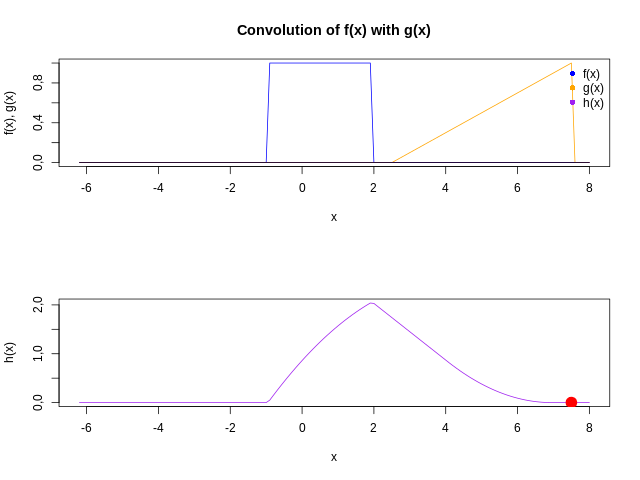
\includegraphics[width=11cm]{plots/conv_animations/conv_anim_28.png}}%
         \only<29>{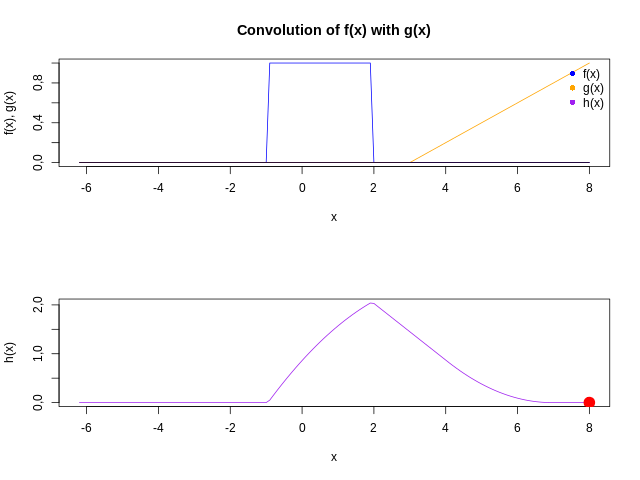
\includegraphics[width=11cm]{plots/conv_animations/conv_anim_29.png}}%
 }


%\frame{
%\frametitle{1D Convolution Animation}
%    \center
%        \only<1>{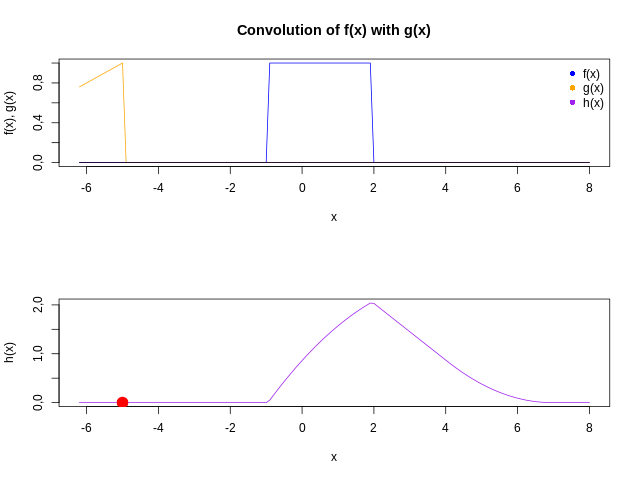
\includegraphics[width=11cm]{plots/conv_animations/conv_anim_3.png}}%
%        \only<2>{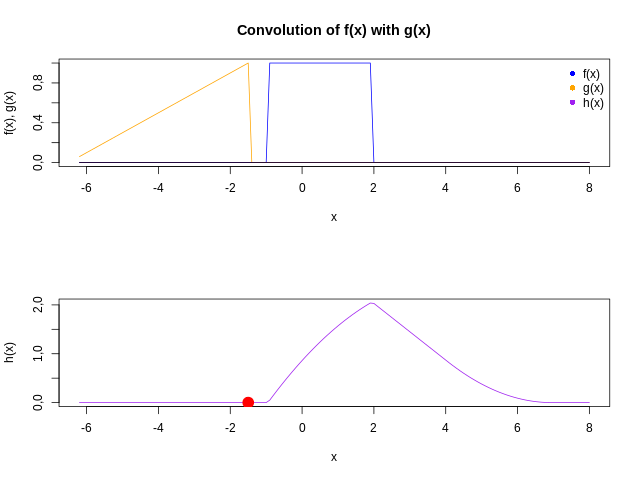
\includegraphics[width=11cm]{plots/conv_animations/conv_anim_10.png}}%
%        \only<3>{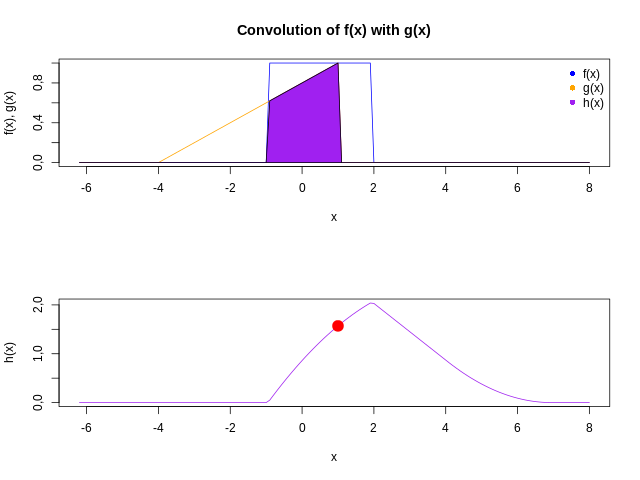
\includegraphics[width=11cm]{plots/conv_animations/conv_anim_15.png}}%
%        \only<4>{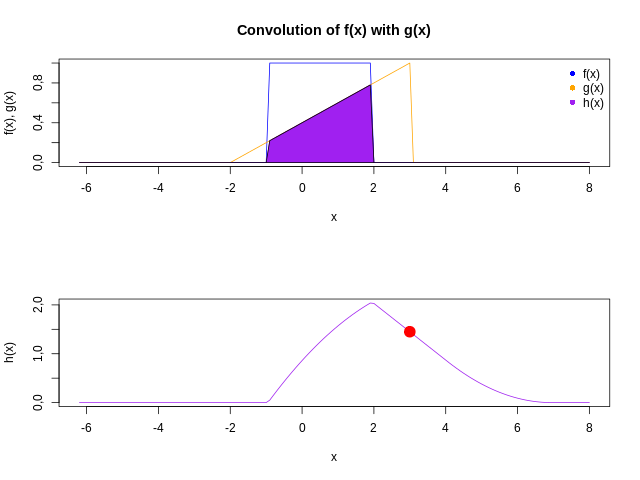
\includegraphics[width=11cm]{plots/conv_animations/conv_anim_19.png}}%
%        \only<5>{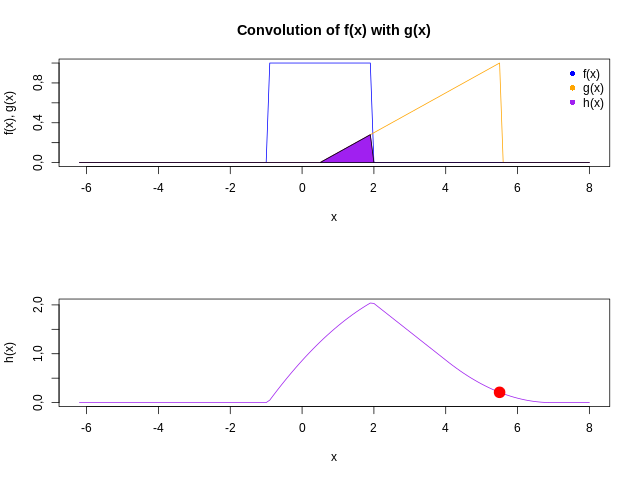
\includegraphics[width=11cm]{plots/conv_animations/conv_anim_24.png}}%
%        \only<6>{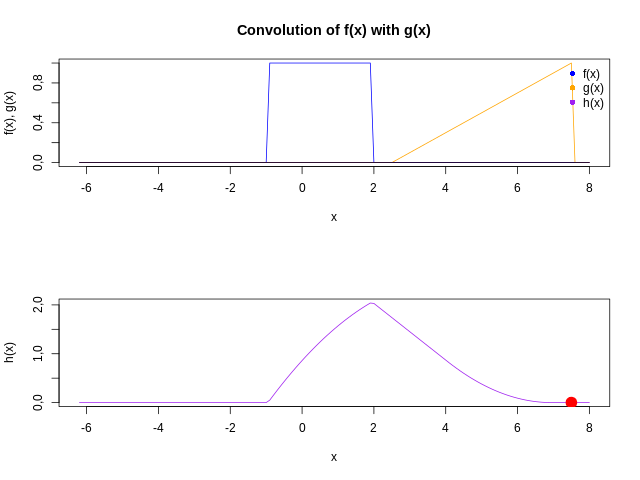
\includegraphics[width=11cm]{plots/conv_animations/conv_anim_28.png}}%
%}

%%%%%%%%%%%%%%%%%%%%%%%%%%%%%%%%%%%%%%%%%%%%%%%%%%%%%%%%%%%%%%%%%%

\frame{
\frametitle{Discretization}

    \begin{itemize}
        \item Discretization for one-dimensional input: \\
            \begin{equation*}
                \begin{split}
                    h(i) &= (f \ast g)(i) = \sum_{x} f(x)g(i-x)
                \end{split}
            \end{equation*}
        \item Discretization for 2D images:
            \begin{itemize}
                \item $\mathcal{I} \in \mathcal{R}^2$ contains two dimensions
                \item Use 2D Kernel $\mathcal{G}$ as well to yield feature map $\mathcal{H}$:
                \begin{equation*}
                    \begin{split}
                        H(i, j) &= (\mathcal{I} \ast \mathcal{G})(i, j) = \sum_{x} \sum_{y} \mathcal{I}(x, y) \mathcal{G}(i-x, j-y) \\
                        \text{where } x, y &:= \text{indices $\mathcal{I}$ and $\mathcal{G}$} \\
                        \text{and } i, j &:= \text{indices elements in } \mathcal{H} \\
                        \end{split}
                \end{equation*}
            \end{itemize}
    \end{itemize}

}

%%%%%%%%%%%%%%%%%%%%%%%%%%%%%%%%%%%%%%%%%%%%%%%%%%%%%%%%%%%%%%%%%%
\begin{vbframe}{Properties of the Convolution}
    \begin{itemize}
        \item Commutativity:
        $$ f \ast g = g \ast f$$
        \item Associativity:
        $$ (f \ast g) \ast h = f \ast (g \ast h)$$
        \item Distributivity:
        $$ f \ast (g + h) = f\ast g + f \ast h$$ 
        $$ \alpha (f \ast g) = (\alpha f) \ast g \text{ for scalar } \alpha$$ 
        \item Differentiability:
        $$ \frac{\partial (f\ast g)(x)}{\partial x_i} = \frac{\partial f(x)}{\partial x_i}\ast g(x) = \frac{\partial g(x)}{\partial x_i} \ast f(x)$$ \\
        $ \rightarrow (f\ast g)(x)$ is as many times differentiable as the max of $g(x)$ and $f(x)$.
    \end{itemize}
\end{vbframe}
%%%%%%%%%%%%%%%%%%%%%%%%%%%%%%%%%%%%%%%%%%%%%%%%%%%%%%%%%%%%%%%%%%
%%%%%%%%%%%%%%%%%%%%%%%%%%%%%%%%%%%%%%%%%%%%%%%%%%%%%%%%%%%%%%%%%%

\begin{vbframe}{Related operations}
    \begin{itemize}
        \item Convolution is strongly related to two other mathematical operators:
        \begin{enumerate}
            \item Fourier transform via the Convolution Theorem
            \item Cross correlation
        \end{enumerate}
    \end{itemize}
\end{vbframe}

%% nice explanation here: https://www.quora.com/How-are-neural-networks-related-to-Fourier-transforms
\begin{vbframe}{Convolution Theorem}
    \begin{itemize}
        \item  Fourier transform of the convolution of two functions can be expressed as the product of their Fourier transforms:
        $$ 
            \mathcal{F} \{ f\ast g\} = \mathcal{F} \{f\}\mathcal{F} \{g\}
        $$
        \item Transformation of a signal from time to frequency domain.
        \item Convolution in the time domain is equivalent to multiplication in frequency domain.
        \item The computationally fastest way to compute a convolution is therefore taking the Fourier inverse of the multiplication of the Fourier-transformed input and filter function :
        $$
            (f \ast g)(t) = \mathcal{F}^{-1}\{\mathcal{F} \{f(t)\} \mathcal{F} \{g(t)\}\}
        $$
    \end{itemize}
\end{vbframe}

 \begin{vbframe}{Convolution Theorem - Proof}
     \begin{equation*}
         \begin{split}
             \widehat{(f \ast g)(t)} &= \int_{-\infty}^\infty exp(-2 \pi i \omega t) \Big[ \int_{-\infty}^\infty f(\tau) g(t-\tau)d\tau \Big] \\
             & = \int_{-\infty}^\infty \int_{-\infty}^\infty exp(-2 \pi i \omega t) f(\tau)g(t-\tau)d\tau dt \\
             & \overset{Fubini}{=} \int_{-\infty}^\infty \Big[ \int_{-\infty}^\infty exp(-2 \pi i \omega t) f(\tau) g(t-\tau ) dt  \Big] d\tau \\
             & \overset{f(\tau) \perp t}{=} \int_{-\infty}^\infty f(\tau) \Big[ \int_{-\infty}^\infty exp(-2 \pi i \omega t) g(t-\tau) dt \Big]d \tau \\
             & \overset{u = t - \tau}{=} \int_{-\infty}^\infty f(\tau) \Big[ \int_{-\infty}^\infty exp(-2\pi i \omega \tau) exp(-2 \pi i \omega u) g(u) du \Big] d\tau \\
             & = \int_{-\infty}^\infty exp(-2 \pi i \omega \tau) f(\tau) \Big[ \int_{-\infty}^\infty exp(-2 \pi i \omega u) g(u) du \Big] d \tau \\
             & \overset{Fubini}{=} ...
         \end{split}
     \end{equation*}
 \end{vbframe}
 
 \begin{vbframe}{Convolution Theorem - Proof}
     \begin{equation*}
         \begin{split}
             &... \int_{-\infty}^\infty exp(-2 \pi i \omega \tau) f(\tau) d\tau \int_{-\infty}^\infty exp(-2 \pi i \omega u) g(u) du \\
             &= \hat{f(t)}\hat{g(t)}
         \end{split}
     \end{equation*}
 \end{vbframe}

%%%%%%%%%%%%%%%%%%%%%%%%%%%%%%%%%%%%%%%%%%%%%%%%%%%%%%%%%%%%%%%%%%
%%%%%%%%%%%%%%%%%%%%%%%%%%%%%%%%%%%%%%%%%%%%%%%%%%%%%%%%%%%%%%%%%%

\begin{vbframe}{Cross Correlation}
    \begin{itemize}
        \item Measurement for similarity of two functions $f(x), g(x)$.
        \item More specifically, at which position are the two functions most similar to each other? Where does the pattern of $g(x)$ match $f(x)$ the best?
        \item Intuition:
        \begin{itemize}
                \item Slide with $g(x)$ over $f(x)$ and at each discrete step compute the sum of the product of their elements.
                \item When peaks of both functions are aligned, the product of high (positive or negative) values will lead to high sums.
                \item Thus, both functions are most similar at points with equal peaks.
        \end{itemize}
    \end{itemize}
\framebreak
    \begin{itemize}
        \item Definition: \\
            \begin{equation*}
                \begin{split}
                    h(i) &= (f \star g)(i) = \int_{-\infty}^{\infty} f(x)g(i+x)dx \\
                    \text{where } f(x)&: \text{input function} \\
                    \text{and } g(x)&: \text{weighting function, kernel} \\
                    \text{and } h(i)&: \text{output function, feature map elements} \\
                    \text{for } f, g &\in \mathcal{R}^{d} \mapsto h \in \mathcal{R}^{d}
                \end{split}
            \end{equation*}
    \end{itemize}
\framebreak 
    \begin{itemize}
        \item Discrete formulation:
            \begin{equation*}
                h(i) = (f \star g)(i) = \sum_{x = -\infty}^{\infty} f(x)g(i+x)
            \end{equation*}
        \item Thus:
            \begin{equation*}
                    f(i) \star g(i) = f(-i) \ast g(i)
            \end{equation*}
        \item Remember: $\ast$ is used for convolution and $\star$ for cross correlation.
        \item Similar formulation as the convolution despite the flipped filter function in the convolutional kernel .
    \end{itemize}
\framebreak
    \begin{itemize}
        \item This operation also works in 2 dimensions
        \item The difference w.r.t. the convolution are the positive iterators in the sum:
        \begin{equation*}
                    \begin{split}
                        H(i, j) &= (\mathcal{I} \star \mathcal{G})(i, j) = \sum_{x} \sum_{y} \mathcal{I}(x, y) \mathcal{G}(i+x, j+y) \\
                        \text{where } x, y &:= \text{indices $\mathcal{I}$ and $\mathcal{G}$} \\
                        \text{and } i, j &:= \text{indices elements in } \mathcal{H} \\
                        \end{split}
                \end{equation*}
    \end{itemize}
\framebreak
    \begin{figure}
        \centering
        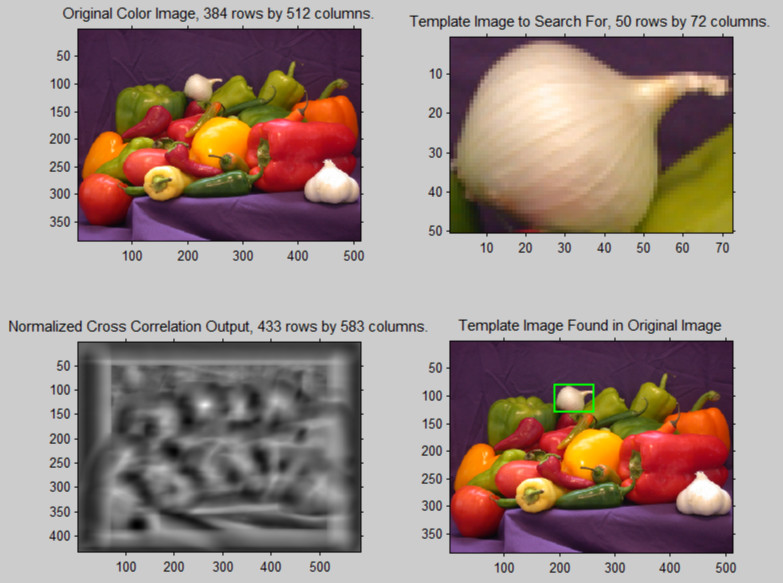
\includegraphics[width=9cm]{plots/other/template_match.png}
        \caption{Cross-correlation used to detect a template (onion) in an image. Cross correlation peaks (white) at the position where template and input match best.}
    \end{figure}
\end{vbframe}

\begin{vbframe}{Cross Correlation}
    % nice video
    \begin{itemize}
        \item From the following animation we see that
        \begin{itemize}
            \item Kernel is not flipped as opposed to the convolution.
            \item Cross-Correlation peaks, where the filter matches the signal the most.    
        \end{itemize}
        \item In some frameworks, Cross-Correlation is implemented instead of the convolution due to
        \begin{itemize}
            \item better computational performance.
            \item similar properties, as the kernel weights are learned throughout the training process.
        \end{itemize}
    \end{itemize}
\end{vbframe}
 
 \frame{
 \frametitle{1D Cross Correlation Animation}
     \center
         \only<1>{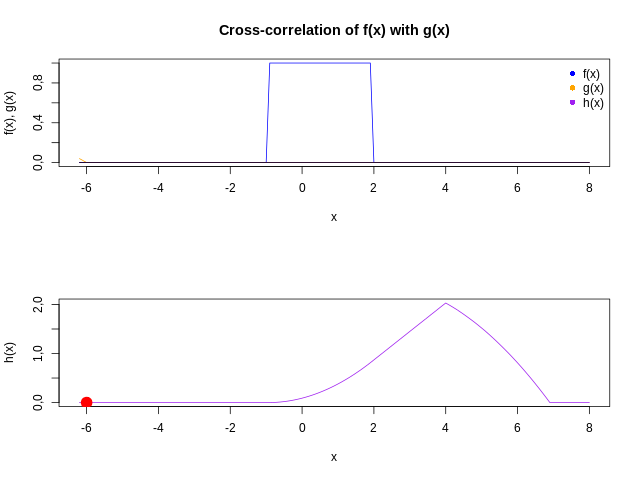
\includegraphics[width=11cm]{plots/xcorrel_animations/xcorrel_anim_1.png}}%
         \only<2>{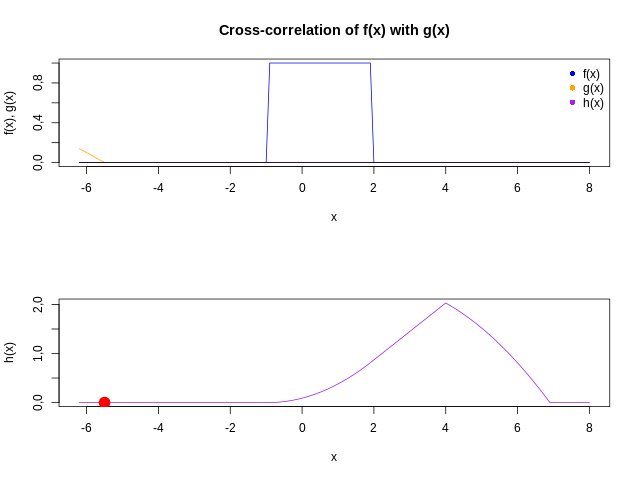
\includegraphics[width=11cm]{plots/xcorrel_animations/xcorrel_anim_2.png}}%
         \only<3>{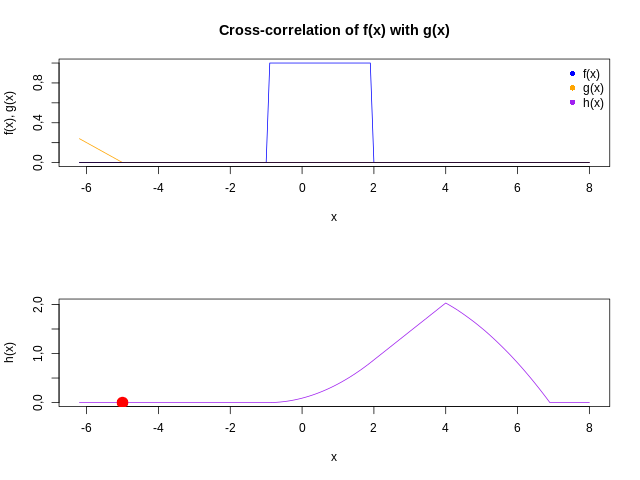
\includegraphics[width=11cm]{plots/xcorrel_animations/xcorrel_anim_3.png}}%
         \only<4>{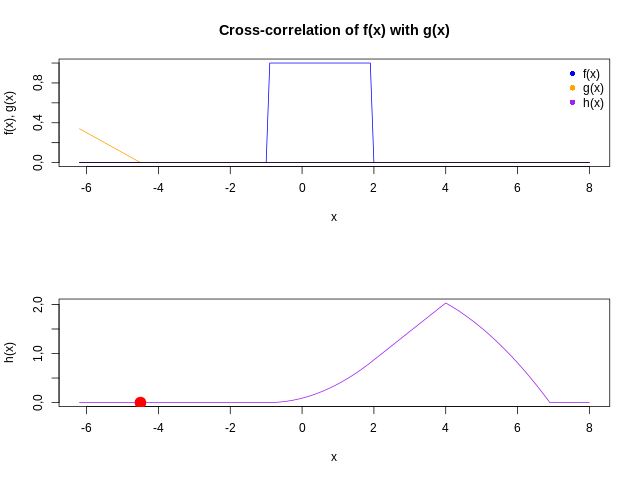
\includegraphics[width=11cm]{plots/xcorrel_animations/xcorrel_anim_4.png}}%
         \only<5>{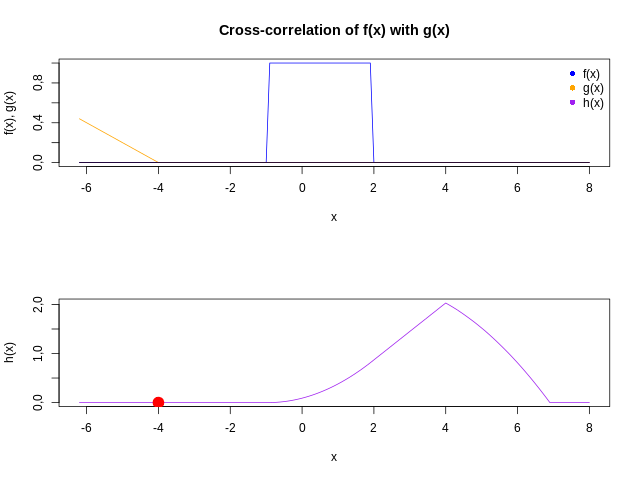
\includegraphics[width=11cm]{plots/xcorrel_animations/xcorrel_anim_5.png}}%
         \only<6>{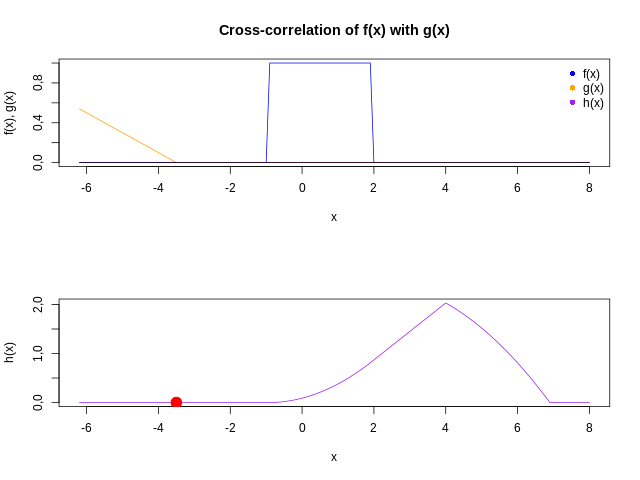
\includegraphics[width=11cm]{plots/xcorrel_animations/xcorrel_anim_6.png}}%
         \only<7>{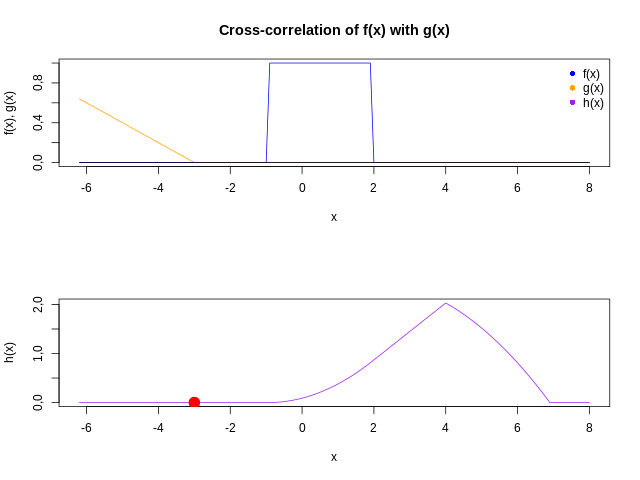
\includegraphics[width=11cm]{plots/xcorrel_animations/xcorrel_anim_7.png}}%
         \only<8>{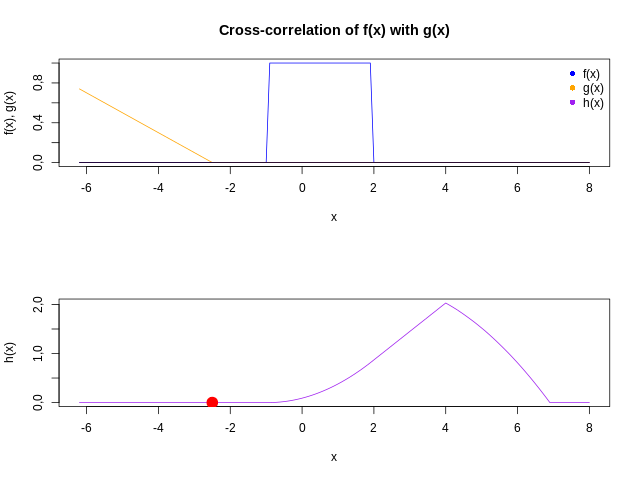
\includegraphics[width=11cm]{plots/xcorrel_animations/xcorrel_anim_8.png}}%
         \only<9>{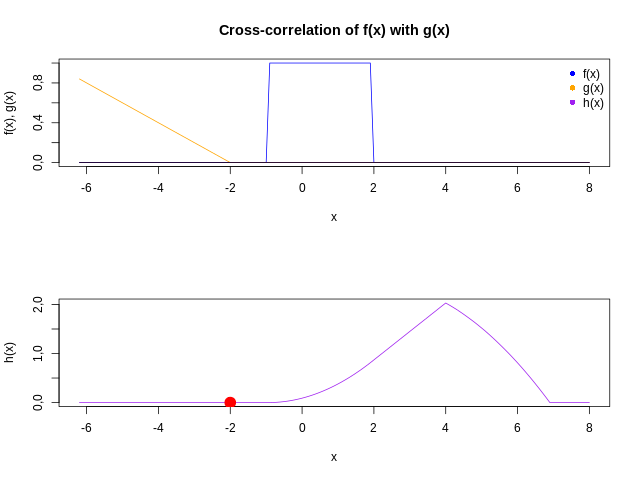
\includegraphics[width=11cm]{plots/xcorrel_animations/xcorrel_anim_9.png}}%
         \only<10>{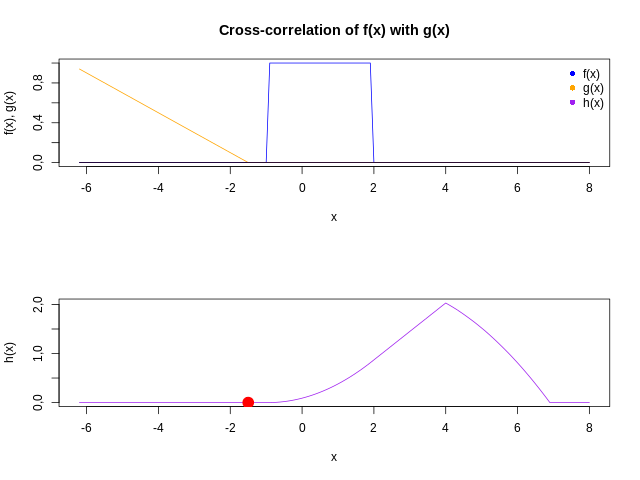
\includegraphics[width=11cm]{plots/xcorrel_animations/xcorrel_anim_10.png}}%
         \only<11>{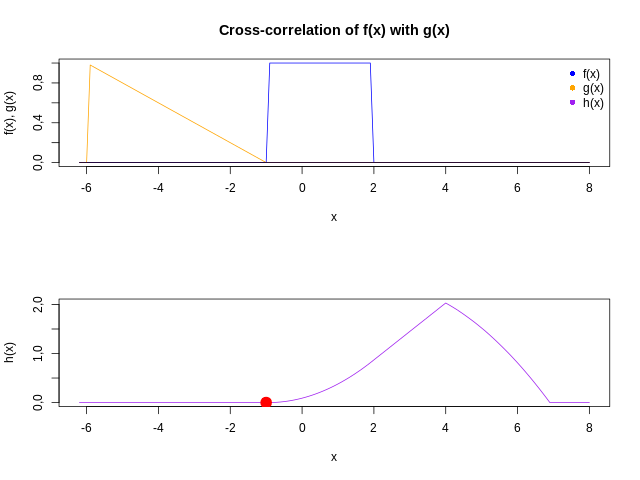
\includegraphics[width=11cm]{plots/xcorrel_animations/xcorrel_anim_11.png}}%
         \only<12>{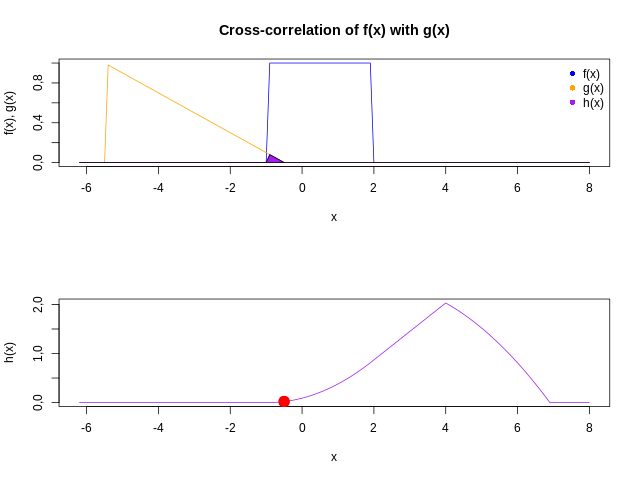
\includegraphics[width=11cm]{plots/xcorrel_animations/xcorrel_anim_12.png}}%
         \only<13>{\includegraphics[width=11cm]{plots/xcorrel_animations/xcorrel_anim_13.png}}%
         \only<14>{\includegraphics[width=11cm]{plots/xcorrel_animations/xcorrel_anim_14.png}}%
         \only<15>{\includegraphics[width=11cm]{plots/xcorrel_animations/xcorrel_anim_15.png}}%
         \only<16>{\includegraphics[width=11cm]{plots/xcorrel_animations/xcorrel_anim_16.png}}%
         \only<17>{\includegraphics[width=11cm]{plots/xcorrel_animations/xcorrel_anim_17.png}}%
         \only<18>{\includegraphics[width=11cm]{plots/xcorrel_animations/xcorrel_anim_18.png}}%
         \only<19>{\includegraphics[width=11cm]{plots/xcorrel_animations/xcorrel_anim_19.png}}%
         \only<20>{\includegraphics[width=11cm]{plots/xcorrel_animations/xcorrel_anim_20.png}}%
         \only<21>{\includegraphics[width=11cm]{plots/xcorrel_animations/xcorrel_anim_21.png}}%
         \only<22>{\includegraphics[width=11cm]{plots/xcorrel_animations/xcorrel_anim_22.png}}%
         \only<23>{\includegraphics[width=11cm]{plots/xcorrel_animations/xcorrel_anim_23.png}}%
         \only<24>{\includegraphics[width=11cm]{plots/xcorrel_animations/xcorrel_anim_24.png}}%
         \only<25>{\includegraphics[width=11cm]{plots/xcorrel_animations/xcorrel_anim_25.png}}%
         \only<26>{\includegraphics[width=11cm]{plots/xcorrel_animations/xcorrel_anim_26.png}}%
         \only<27>{\includegraphics[width=11cm]{plots/xcorrel_animations/xcorrel_anim_27.png}}%
         \only<28>{\includegraphics[width=11cm]{plots/xcorrel_animations/xcorrel_anim_28.png}}%
         \only<29>{\includegraphics[width=11cm]{plots/xcorrel_animations/xcorrel_anim_29.png}}%
 }

%\frame{
%\frametitle{1D Cross Correlation Animation}
%    \center
%        \only<1>{\includegraphics[width=11cm]{plots/xcorrel_animations/xcorrel_anim_3.png}}%
%        \only<2>{\includegraphics[width=11cm]{plots/xcorrel_animations/xcorrel_anim_10.png}}%
%        \only<3>{\includegraphics[width=11cm]{plots/xcorrel_animations/xcorrel_anim_15.png}}%
%        \only<4>{\includegraphics[width=11cm]{plots/xcorrel_animations/xcorrel_anim_19.png}}%
%        \only<5>{\includegraphics[width=11cm]{plots/xcorrel_animations/xcorrel_anim_24.png}}%
%        \only<6>{\includegraphics[width=11cm]{plots/xcorrel_animations/xcorrel_anim_28.png}}%
%}


%%%%%%%%%%%%%%%%%%%%%%%%%%%%%%%%%%%%%%%%%%%%%%%%%%%%%%%%%%%%%%%%%%
%%%%%%%%%%%%%%%%%%%%%%%%%%%%%%%%%%%%%%%%%%%%%%%%%%%%%%%%%%%%%%%%%%
\begin{vbframe}{Cross Correlation vs. Convolution}
    \begin{figure}
        \centering
        \includegraphics[width=4cm]{plots/xcorrel_animations/conv_xcorrel.png}
        \caption{Comparison of convolution and cross-correlation}
    \end{figure}
    
    \begin{itemize}
    \item Cross correlation is not commutative
    \item but often implemented instead of convolution in the practice.
    \end{itemize}
\end{vbframe}


%%%%%%%%%%%%%%%%%%%%%%%%%%%%%%%%%%%%%%%%%%%%%%%%%%%%%%%%%%%%%%%%%%
%%%%%%%%%%%%%%%%%%%%%%%%%%%%%%%%%%%%%%%%%%%%%%%%%%%%%%%%%%%%%%%%%%


\endlecture
\end{document}